\documentclass{article}

% Language setting Replace `english' with e.g. `spanish' to change the document
% language
\usepackage[english]{babel}
\usepackage{mathtools}
% Set page size and margins Replace `letterpaper' with `a4paper' for UK/EU
% standard size
\usepackage[letterpaper,top=2cm,bottom=2cm,left=3cm,right=3cm,marginparwidth=1.75cm]{geometry}

% Useful packages
\usepackage{amsmath}
\usepackage{graphicx}
\usepackage[colorlinks=true, allcolors=blue]{hyperref}

\title{Halfar Model Numerics Example}
\author{Drisana Iverson (dmosaphir@sift.net) and Dan Bryce (dbryce@sift.net)}

\begin{document}
\maketitle


\section{Discretized PDEs as continuous Petrinets}

We discretize and solve PDEs expressed with partial derivatives $\dfrac{\partial
        u}{\partial t}$ and  $\dfrac{\partial u}{\partial x}$ over time $t$ and space
$x$ by encoding discrete approximations of the PDE as continuous Petrinets.  Our
method relies upon the semantics of continuous Petrinets wherein transitions and
the associated transition rates describe flow along the PDE gradient. A single
Petrinet transition of the form

$$\{u_1\}\xrightarrow{r}\{u_2\}$$

\noindent corresponds to

$$\dfrac{\partial u_1}{\partial t}  = -r \qquad \dfrac{\partial u_2}{\partial t}
    = r$$

\noindent and encodes a flow from $u_1$ to $u_2$ with rate $r$.  Similarly,
partial derivatives

$$\dfrac{\partial u_3}{\partial t} = r_1 + r_2  \qquad \dfrac{\partial
        u_4}{\partial t} = r_1 - r_2$$

\noindent correspond to transitions

$$\{u_4\}\xrightarrow{r_2}\{u_3\} \qquad \{\}\xrightarrow{2 r_1}\{u_3, u_4\}$$

\noindent where the \emph{aggregate} flow rate for each variable is identical to
the partial derivative with respect to time.  We encode discretized PDEs as a
Petrinet, where states correspond to each variable at different spatial points
and the rates encode the partial derivatives.

We define the discretizations of space and time respectively as

\[ u_i^k = u(x_i, t_k) \] where

\[x_i = i\Delta x, \qquad i \in [0, I) \] \[t_k = k\Delta t, \qquad k \in [0,
        K]\]

\noindent Then we refer to the definitions of the partial derivatives with the
function $F$.

\begin{equation} \label{eq:first_deriv_time}
    \dfrac{\partial u}{\partial t}(x_i, t_k)= F_{ut}(x_i,t_k)%\dfrac{u_i^{k+1}-u_i^k}{\Delta t}
\end{equation}

\begin{equation}\label{eq:first_deriv_space}
    \dfrac{\partial u}{\partial x}(x_i, t_k) = F_{ux}(x_i,t_k) %\dfrac{u_{i+1}^{k}-u_{i-1}^k}{2\Delta x}
\end{equation}
\noindent The subscripts identify the partial derivative with respect to $t$ and
$x$, respectively.  We also denote by ${\tt F}$, the discretization of a partial
derivative, for example, the forward derivative:


\begin{equation} \label{eq:discretization}
    \begin{split}
        \dfrac{\partial u}{\partial t}(x_i, t_k)=F_{ut}(x_i,t_k) \approx {\tt F}_{ut}(x_i,t_k) = \dfrac{u_i^{k+1}-u_i^k}{\Delta t}\\
        \dfrac{\partial u}{\partial x}(x_i, t_k) = F_{ux}(x_i,t_k)\approx {\tt F}_{ux}(x_i,t_k) = \dfrac{u_{i+1}^k-u_i^k}{\Delta x}
    \end{split}
\end{equation}

\noindent  In the following, we discretize the definitions of partial
derivatives $F$ by substituting the chosen discretization ${\tt F}$. While
Equation \ref{eq:discretization} illustrates using a particular approximation of
the partial derivative, this choice is an arbitrary, but important, decision.
We discuss several possible definitions in the following section.  

Solving for
$u_i^{k+1}$ in Equation \ref{eq:discretization} allows us to define:

\begin{equation} \label{eq:step-update}
    \begin{split}
        u_i^{k+1}& = u_i^k + {\tt F}_{ut}(x_i,t_k)\Delta t
    \end{split}
\end{equation}

\noindent where ${\tt F}$ is the discretization of an arbitrary expression $F$
that includes, for example, additional partial derivatives.  If the expression
$F_{ut}(x_i,t_k)$  includes a partial derivative term $F'$, then we substitute
${\tt F'}$, recursively.  For example,  the advection operator applied to a
vector field $a$: \[({\bf u}\cdot \nabla) a = -u\dfrac{\partial a}{\partial
        x}-v\dfrac{\partial a}{\partial  y}-w\dfrac{\partial a}{\partial  z}\] defines
the equation:
\[\dfrac{\partial a}{\partial t} = - u\dfrac{\partial a}{\partial x} -
    v\dfrac{\partial a}{\partial y} - w\dfrac{\partial a}{\partial z}  \] The
partial deriviative of $a$ wrt. to time at point $p_i = (x_{i_1}, y_{i_2},
    z_{i_3})$ and time $t_k$ is:

\begin{equation} \label{eq:advection-partials}
    \begin{split}
        \dfrac{\partial a}{\partial t}(p_i, t_k) &= F_{at}(p_i, t_k) \\
        &= - u F_{ax}(p_i, t_k) \\
        &\quad - v F_{ay}(p_i, t_k) \\
        &\quad - w F_{az}(p_i, t_k)
    \end{split}
\end{equation}

\noindent Discretizing $F_{at}$ involves substituting ${\tt F}_{ax}$, ${\tt
            F}_{ay}$, and ${\tt F}_{az}$ so that:

\begin{equation} \label{eq:advection-discretization}
    \begin{split}
        F_{at}(p, t_k) \approx {\tt F}_{at}(p_i, t_k)
        = - u {\tt F}_{ax}(p_i, t_k)
        - v {\tt F}_{ay}(p_i, t_k)
        - w {\tt F}_{az}(p_i, t_k)
    \end{split}
\end{equation}

Expanding each derivative term ${\tt F}$ will result in the expression:

\begin{equation} \label{eq:advection-discretization-expansion}
    \begin{split}
        {\tt F}_{at}(p_i, t_k)& = - u {\tt F}_{ax}(p_i, t_k)
        - v {\tt F}_{ay}(p_i, t_k)
        - w {\tt F}_{az}(p_i, t_k)\\
        \dfrac{a^{k+1}_{i} - a^{k}_{i}}{\Delta t} &= -u\dfrac{a^{k}_{i_{x^+}} - a^{k}_{i}}{\Delta x} -v\dfrac{a^{k}_{i_{y^+}} - a^{k}_{i}}{\Delta y} -w\dfrac{a^{k}_{i_{z^+}} - a^{k}_{i}}{\Delta z}
    \end{split}
\end{equation}

\noindent where $i_{x^+}$ corresponds to  $(x_{i_1+1}, y_{i_2}, z_{i_3})$, and
similarly for $i_{y^+}$ and $i_{z^+}$. Solving
\ref{eq:advection-discretization-expansion} for $a^{k+1}_{i}$ provides a
state-update expression:

\begin{equation} \label{eq:advection-discretization-expansion-update}
    \begin{split}
        a^{k+1}_{i}  = a^{k}_{i} +  \left(-u\dfrac{a^{k}_{i_{x^+}} - a^{k}_{i}}{\Delta x} -v\dfrac{a^{k}_{i_{y^+}} - a^{k}_{i}}{\Delta y} -w\dfrac{a^{k}_{i_{z^+}} - a^{k}_{i}}{\Delta z}\right) \Delta t
    \end{split}
\end{equation}

% \[F_{ut}(x_i,t_k) = -a\dfrac{\partial u}{\partial x} -a\dfrac{\partial
%     v}{\partial y}\] (as ), then \[F_{ux}' = -a\dfrac{\partial u}{\partial
%     x}\] \[{\tt F}_{ux}' = -a\dfrac{u_{i}^k - u_{i-1}^k}{\Delta x}\] and
%     \[u_i^{k+1} \approx u_i^k + -a\dfrac{u_{i}^k - u_{i-1}^k}{\Delta x}\Delta
%     t\]


% This discretization scheme allows us to define $F_{ut}(x_i,t_k)$ in Equation
% \ref{eq:step-update} as linear combination because the discretization ${\tt
% F}'$ of each term $F'$ is a linear combination.  From the example above, we
% can rewrite it as follows:

% \begin{equation} \label{eq:rate-equation} \begin{split} u_i^{k+1}& \approx
%     u_i^k + -a\dfrac{u_{i}^k - u_{i-1}^k}{\Delta x}\Delta t\\
%         & = u_i^k + \left(\dfrac{-au_{i}^k }{\Delta x}-
%         \dfrac{-au_{i-1}^k}{\Delta x}\right)\Delta t\\
%         & = u_i^k + \left(r' - r \right)\Delta t \end{split} \end{equation}

% \noindent  In general, the terms may be another expression obtained by
% discretizing a partial deriviative with respect to $x$. We illustrate several
% such examples below.

\noindent Our main observation is that the state-update expression can be
expressed as a linear combination of terms (which we refer to as rates $r$):

\begin{equation} \label{eq:petri-semantics}
    \begin{split}
        a^{k+1}_{i}  = & a^{k}_{i} +  \left(-u\dfrac{a^{k}_{i_{x^+}} - a^{k}_{i}}{\Delta x} -v\dfrac{a^{k}_{i_{y^+}} - a^{k}_{i}}{\Delta y} -w\dfrac{a^{k}_{i_{z^+}} - a^{k}_{i}}{\Delta z}\right) \Delta t\\
        = &  a^{k}_{i} +  \left(-u\dfrac{a^{k}_{i_{x^+}}}{\Delta x} -u\dfrac{- a^{k}_{i}}{\Delta x} -v\dfrac{a^{k}_{i_{y^+}} }{\Delta y} -v\dfrac{ - a^{k}_{i}}{\Delta y} -w\dfrac{a^{k}_{i_{z^+}} }{\Delta z} -w\dfrac{ - a^{k}_{i}}{\Delta z}\right) \Delta t\\
        = &  a^{k}_{i} +  \left(r_{x^+} -r_x  + r_{y^+} -r_y + r_{z^+} -r_z\right) \Delta t
    \end{split}
\end{equation}

\noindent Rewriting Equation \ref{eq:petri-semantics}, we can recover the
partial derivative expressed in terms of rates:

\begin{equation} \label{eq:petri-semantics-rates}
    \begin{split}
        \dfrac{a^{k+1}_{i}-a^{k}_{i}}{\Delta t}
        &=     r_{x^+} -r_x  + r_{y^+} -r_y + r_{z^+} -r_z\\
        & \approx   \dfrac{\partial a}{\partial t}(p_i, t_k)
    \end{split}
\end{equation}

Petrinets expressing mass action kinetics use the same format, whereby positive
terms are the rates associated with incoming transitions and negative, outgoing
transitions.  We denote by $src \xrightarrow{r} dest$ a transition from states
in $src$ to states in $dest$ with rate $r$.  We express Equation
\ref{eq:petri-semantics-rates} as the transitions:

\begin{equation} \label{eq:petri-semantics-transitions}
    \begin{split}
        \{a_{i_{x^+}}\}&\xrightarrow{r_{x^+}}\{a_{i}\}\\
        \{a_{i}\}&\xrightarrow{r_{x}}\{a_{i_{x^-}}\}\\
        \{a_{i_{y^+}}\}&\xrightarrow{r_{y^+}}\{a_{i}\}\\
        \{a_{i}\}&\xrightarrow{r_{y}}\{a_{i_{y^-}}\}\\
        \{a_{i_{z^+}}\}&\xrightarrow{r_{z^+}}\{a_{i}\}\\
        \{a_{i}\}&\xrightarrow{r_{z}}\{a_{i_{z^-}}\}
    \end{split}
\end{equation}

\noindent where $i_{x^-}$ corresponds to  $(x_{i_1-1}, y_{i_2}, z_{i_3})$, and
similarly for $i_{y^-}$ and $i_{z^-}$.  The transitions refer to these neighboring locations because they share common rate terms.  Aggregating the transitions allows us to express $\dfrac{\partial a}{\partial t}$ for all locations.

We handle boundary conditions implicitly by using transitions with an empty $src$ or $dest$, and a rate that substitutes references to the value of boundary locations with an expression.  For example, if $a_i^k$ appears in a rate expression and location $i$ is a boundary location (e.g., $i = -1$ or $i= I$, in the one dimensional case), then we replace $a_i^k$ with the boundary condition $b(a, t)$.  The Petrinet does not represent boundary locations with state variables because, otherwise, the semantics for the Petrinet would cause those state variables to be updated.  It is sufficient to leak the boundary rate expressions into locations on the upper boundaries and out from locations on the lower boundaries to ensure the appropriate rate terms impact the state variables with transitions of the form $\{\}\xrightarrow{r_{b}}\{a_{I-1}\}$ (upper) and $\{a_0\}\xrightarrow{r_{b}}\{\}$ (lower).


\section{Discretizing Partial Derivatives}

We consider three primary methods for computing partial derivatives from a
discretization: forward, backward, and centered.  The definitions in Equation
\ref{eq:discretization} correspond to the forward derivative, calculating the
derivative at $u_i^k$ by considering the next greater point along the respective
dimension, $u_{i+1}^k$ or $u_i^{k+1}$.  We define the backward derivative as:

\begin{equation} \label{eq:discretization-backward}
    \begin{split}
        {\tt F}_{ut}(x_i,t_k)= \dfrac{u_i^{k}-u_i^{k-1}}{\Delta t}\\
        {\tt F}_{ux}(x_i,t_k) = \dfrac{u_{i}^k-u_{i-1}^k}{\Delta x}
    \end{split}
\end{equation}

\noindent and the centered derivative as:

\begin{equation} \label{eq:discretization-centered}
    \begin{split}
        {\tt F}_{ut}(x_i,t_k)= \dfrac{u_i^{k+1}-u_i^{k-1}}{2\Delta t}\\
        {\tt F}_{ux}(x_i,t_k) = \dfrac{u_{i+1}^k-u_{i-1}^k}{2\Delta x}
    \end{split}
\end{equation}

\noindent The primary difference between these methods of calculating the
derivative is how the Petrinet transitions connect the states.

\section{Examples}

We illustrate several examples from climate modeling to show how to transform a
PDE model into a Petrinet.

\subsection{Halfar Equation}

The original Halfar dome equation is given by

\begin{equation}\label{eq:halfar-original}\dfrac{\partial h}{\partial t} = \dfrac{2}{n+2}A(\rho g)^n \dfrac{\partial}{\partial x} \left(\dfrac{\partial h}{\partial x}\left|\dfrac{\partial h}{\partial x}\right|^{n-1} h^{n+2}\right).\end{equation}

\noindent Substituting $\Gamma = \dfrac{2}{n+2}A(\rho g)^n$ (this is a constant) and $n=3$ (also a constant), we get

\begin{equation}\label{eq:halfar}\dfrac{\partial h}{\partial t} = \Gamma \dfrac{\partial}{\partial x} \left(\dfrac{\partial h}{\partial x}\left|\dfrac{\partial h}{\partial x}\right|^{2} h^{5}\right).\end{equation}


\noindent We can start by substituting $\dfrac{\partial h}{\partial t}$ with the
forward derivative ${\tt F}_{ut}$ (Equation \ref{eq:discretization}) and
$\dfrac{\partial h}{\partial x}$ with the centered derivative ${\tt F}_{ux}$
(Equation \ref{eq:discretization-centered}):

% \begin{equation}\label{halfar-step-1} \dfrac{h_i^{k+1}-h_i^k}{\Delta t} =
%     \Gamma \dfrac{\partial}{\partial x} \left(\dfrac{h_{i+1}^{k}-h_i^k}{\Delta
%     x} \left|\dfrac{h_{i+1}^{k}-h_i^k}{\Delta x}\right|^2(h_i^k)^5 \right)
%     \end{equation}

\begin{equation}\label{halfar-step-1}
    \dfrac{h_i^{k+1}-h_i^k}{\Delta t} = \Gamma \dfrac{\partial}{\partial x} \left(\dfrac{h_{i+1}^{k}-h_{i-1}^k}{2\Delta x} \left|\dfrac{h_{i+1}^{k}-h_{i-1}^k}{2\Delta x}\right|^2(h_i^k)^5 \right)
\end{equation}


\noindent Then, to simplify the expression, we can define

% \begin{equation}\label{halfar-inner-term} w_i^k =
%     \dfrac{h_{i+1}^{k}-h_i^k}{\Delta x} \left|\dfrac{h_{i+1}^{k}-h_i^k}{\Delta
%     x}\right|^2(h_i^k)^5 \end{equation}


\begin{equation}\label{halfar-inner-term}
    w_i^k =
    \dfrac{h_{i+1}^{k}-h_{i-1}^k}{2\Delta x} \left|\dfrac{h_{i+1}^{k}-h_{i-1}^k}{2\Delta x}\right|^2(h_i^k)^5
\end{equation}

\noindent Substituting Equation \ref{halfar-inner-term}, we get

\begin{equation}\label{halfar-step-2}
    \dfrac{h_i^{k+1}-h_i^k}{\Delta t} = \Gamma \dfrac{\partial}{\partial x} w_i^k
\end{equation}

\noindent We can then use Eq. \ref{eq:discretization-centered} a second time to
get

% \begin{equation}\label{halfar-step-3} \dfrac{h_i^{k+1}-h_i^k}{\Delta t} =
%     \Gamma \left(\dfrac{w_{i+1}^k-w_i^k}{\Delta x}\right) \end{equation}

\begin{equation}\label{halfar-step-3}
    \dfrac{h_i^{k+1}-h_i^k}{\Delta t} = \Gamma \left(\dfrac{w_{i+1}^k-w_{i-1}^k}{2\Delta x}\right)
\end{equation}

\noindent Solving for $h_i^{k+1}$ gives the step update equation:

% \begin{equation}\label{halfar-update} h_i^{k+1} = h_i^k + \Gamma \Delta t
%     \left(\dfrac{w_{i+1}^k-w_i^k}{\Delta x}\right). \end{equation}

\begin{equation}\label{halfar-update}
    h_i^{k+1} = h_i^k + \Gamma \Delta t  \left(\dfrac{w_{i+1}^k-w_{i-1}^k}{2\Delta x}\right).
\end{equation}

% \noindent We will also need to assign values to the initial points $h_i^0$ for
% all spatial points $i$, and the boundary points $h_0^k$ for all time points
% $k$.

\noindent Re-writing equation \ref{halfar-update}, we can define for each $i
    =[0, I)$:

\begin{equation}\label{halfar-petri-update}
    \begin{split}
        h_i^{k+1} &= h_i^k + \left(\dfrac{\Gamma }{2\Delta x}w_{i+1}^k -\dfrac{\Gamma }{2\Delta x}w_{i-1}^k\right)\Delta t\\
        &= h_i^k + (r_{i+1} - r_{i-1}) \Delta t
    \end{split}
\end{equation}

\noindent where we drop the time index $k$ so that

\begin{equation}\label{halfar-petri-rates}
    \begin{split}
        r_i &= \dfrac{\Gamma}{2\Delta x}w_i\\
        &= \dfrac{\Gamma}{2\Delta x}\dfrac{h_{i+1}-h_{i-1}}{2\Delta x} \left|\dfrac{h_{i+1}-h_{i-1}}{2\Delta x}\right|^2(h_i)^5
    \end{split}
\end{equation}

\noindent for $i\in[0, I)$ and $r_{-1} = r_I = B(t)$, where $B(t)$ is the
boundary condition, assumed to be $B(t)= 0$ in the Halfar model.

Expressing Equation \ref{halfar-petri-update} as a Petrinet, results in the
transitions:

% FIXME It would help to expand this transition into equations to show the
% non-intuitive flow that modifies both variables.  Point out that boundaries
% are like vital dynamics.

\begin{align}%\label{halfar-petri-transitions}
    \{h_{i+1}\} & \xrightarrow{r_i} \{h_{i-1}\} \quad : i \in [-1, I]
\end{align}

\noindent where the source and target states are $\{\}$ when $i = I$ or $i=-1$,
respectively.  Figure \ref{fig:halfar-petri} (Centered Difference) illustrates the Petrinet for the
Halfar model when $I=5$.

\begin{figure}[tbh]
    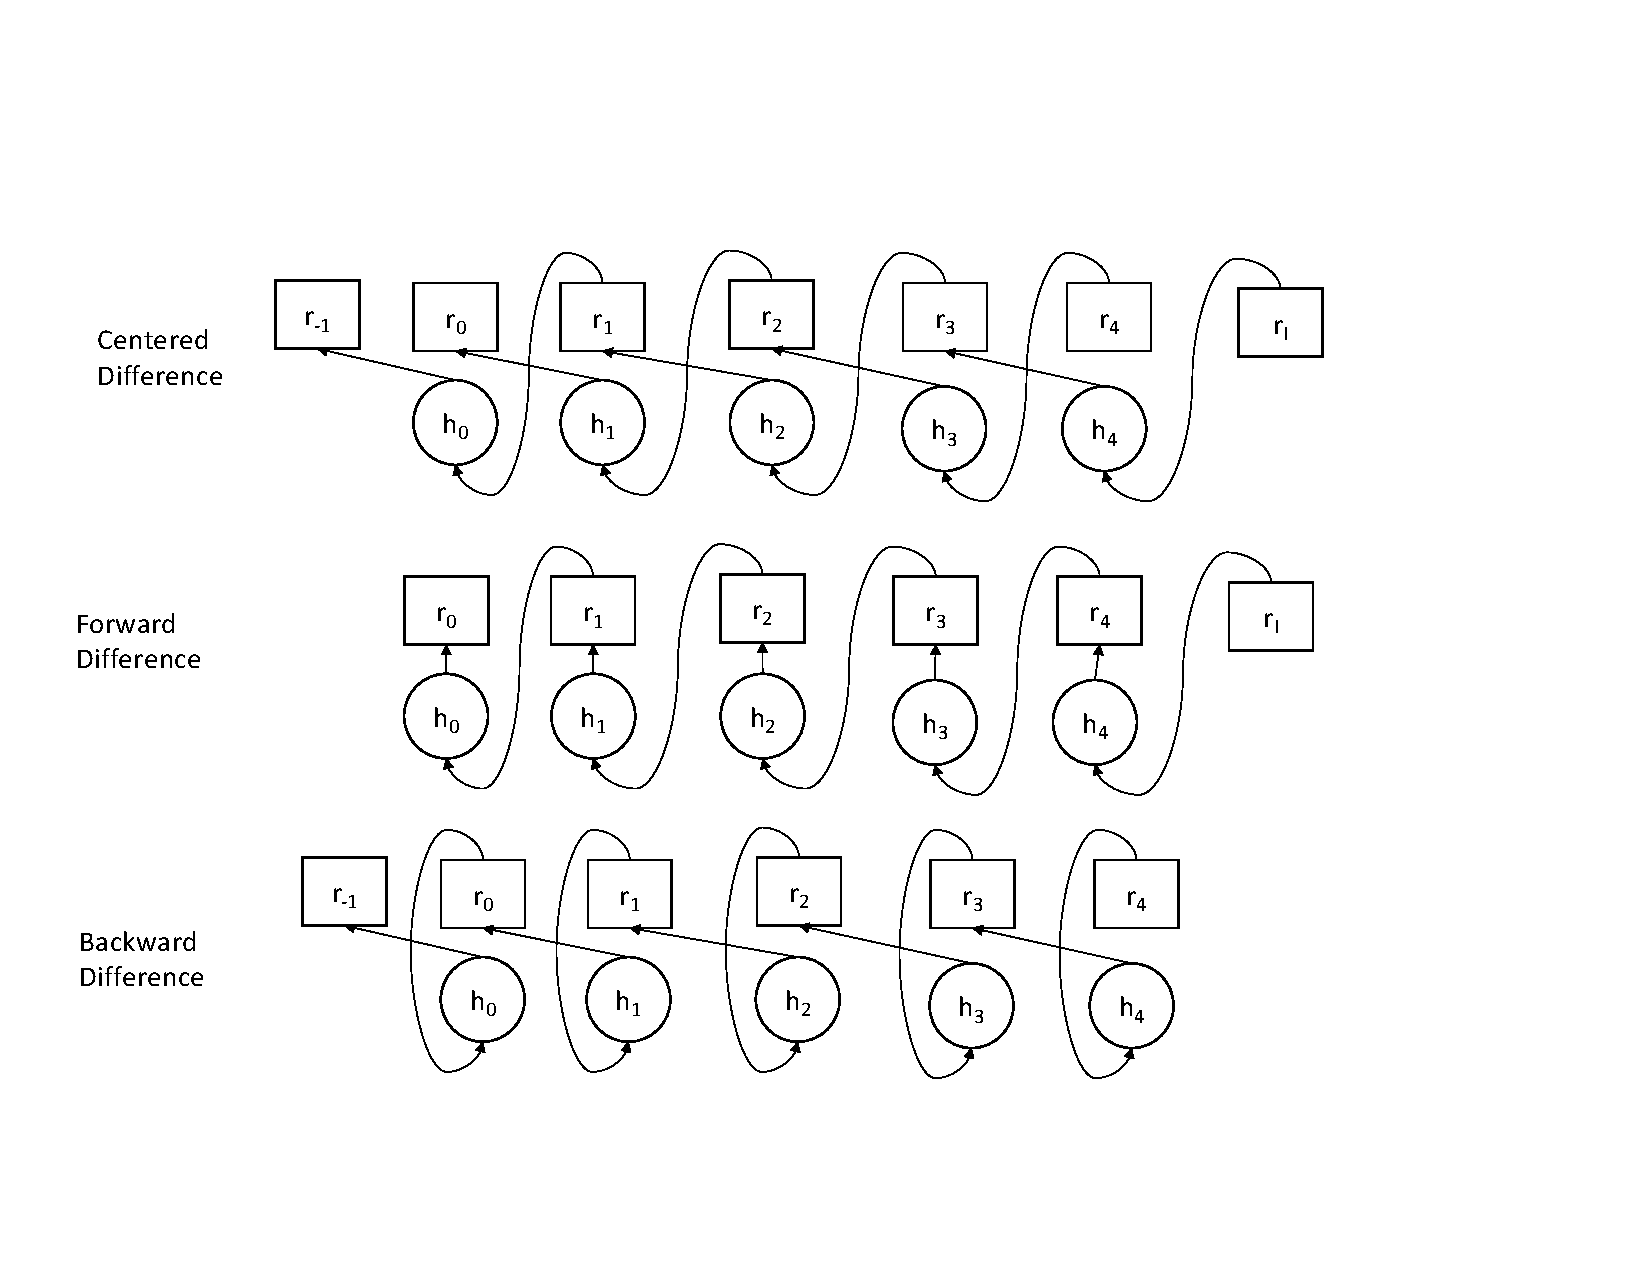
\includegraphics[width=\linewidth]{fig/halfar_petri.pdf}
    \caption{\label{fig:halfar-petri} Petrinets for the Halfar model when $I =
            5$, using different derivatives.  Circles denote states and rectangles denote transitions.}
\end{figure}

\subsection{Advection Equation}

The 1d advection equation (1d version of the Oceananigans equation, from
Scenario 4), is given by

\begin{equation}
    \dfrac{\partial a}{\partial t} + u\dfrac{\partial a}{\partial x} = 0
\end{equation}

% \subsection{Stable discretization for $a > 0$} ref:
% https://indico.ictp.it/event/a06220/session/18/contribution/10/material/0/2.pdf

After substituting the forward derivative for ${\tt F}_{at}$ (Equation
\ref{eq:discretization}) and backward derivative (Equation
\ref{eq:discretization-backward}) for ${\tt F}_{ax}$, the state-update equation
simplifies to:

\begin{equation}
    \begin{split}
        a_i^{k+1} &= a_i^k - u\left(\frac{a_i^k - a_{i-1}^k}{\Delta x}\right)\Delta t\\
        &= u_i^k + \left( \dfrac{-u a_i^k}{\Delta x}  -   \dfrac{-u a_{i-1}^k}{\Delta x} \right)\Delta t\\
        & = a_i^k +  (r_i - r_{i-1})\Delta t\\
    \end{split}
\end{equation}

\noindent where, in the following $r_i = \dfrac{-u a_i }{\Delta x}$ for all $i
    \in {[}0, I)$.

The boundary condition defines:

\begin{equation}
    b(a, t) = 0.0
\end{equation}

The above scheme is stable when $\left|\dfrac{u\Delta t}{\Delta x}\right| \leq
    1$ or equivalently when $\Delta t \leq \dfrac{\Delta x}{|u|}$.

Translating this model to a Petrinet results in transitions of the form:

\begin{equation}
    \begin{split}
        \{a_0\}&\xrightarrow{r_b = 0}\{\}\\
        \{a_1\}&\xrightarrow{r_1 = \dfrac{-u a_1}{\Delta x}}\{a_0\}\\
        &\ldots \\
        \{a_{I-1}\}&\xrightarrow{r_{I-1}= \dfrac{-u a_{I-1}}{\Delta x}}\{a_{I-2}\}\\
        \{\}&\xrightarrow{r_b=0}\{a_{I-1}\}
    \end{split}
\end{equation}

\noindent so that the Petrinet expresses the step updates:
\begin{equation}
    \begin{split}
        a_0^{k+1} &= a_0^k + (r_1 - r_b)\Delta t\\
        a_1^{k+1} &= a_1^k + (r_2 - r_1)\Delta t\\
        &\ldots \\
        a_{I-1}^{k+1}&= a_{I-1}^k + (r_b - r_{I-1})\Delta t
    \end{split}
\end{equation}


% \subsection{Navier-Stokes}

% \begin{equation}
%     \begin{split}
%         u_{ij}^{n+1} = u_{ij}^n - & c_1(u_{ij}^n)^2 + c_1 u_{ij}^n u_{i-1j}^n - c_2 v_{ij}^n u_{ij}^n + c_2 v_{ij}^n u_{ij-1}^n\\
%         & - \dfrac{c_1 }{2\rho}p_{i+1j}^n  + \dfrac{ c_1 }{2\rho }p_{i-1j}^n\\
%         & + \dfrac{ c_1 \nu  }{\Delta x}u_{i+1j}^n - \dfrac{  c_1 \nu}{\Delta x}2u_{ij}^n  + \dfrac{ c_1 \nu}{\Delta x}u_{i-1j}^n\\
%         & + \dfrac{c_2 \nu   }{\Delta y} u_{ij+1}^n - \dfrac{c_2  \nu  }{\Delta y}2u_{ij}^n + \dfrac{c_2 \nu  }{\Delta y}u_{ij-1}^n
%     \end{split}
% \end{equation}

% \begin{equation}
%     \begin{split}
%         v_{ij}^{n+1} = v_{ij}^n - & c_1 u_{ij}^n v_{ij}^n +  c_1 u_{ij}^n v_{i-1j}^n  - c_2(v_{ij}^n)^2  + c_2v_{ij}^n v_{ij-1}^n\\
%         & - \dfrac{ c_2 }{2\rho }p_{ij+1}^n + \dfrac{ c_2 }{2\rho }p_{ij-1}^n\\
%         & + \dfrac{ c_1 \nu   }{\Delta x}v_{i+1j}^n - \dfrac{ c_1 \nu }{\Delta x}2v_{ij}^n   + \dfrac{c_1 \nu  }{\Delta x}v_{i-1j}^n \\
%         & + \dfrac{c_2 \nu  }{\Delta y}v_{ij+1}^n  - \dfrac{c_2 \nu  }{\Delta y}2v_{ij}^n + \dfrac{c_2  \nu  }{\Delta y}v_{ij-1}^n
%     \end{split}
% \end{equation}

% \begin{equation}
%     \begin{split}
%         p_{ij}^{n} = &  c_3 p_{i+1j}^n + c_3 p_{i-1j}^n + c_4 p_{ij+1}^n  + c_4 p_{ij-1}^n +\\
%         & - \dfrac{c_4 \rho   }{2c_1 } u_{i+1j} + \dfrac{c_4 \rho   }{2c_1 }  u_{i-1j}- \dfrac{c_3 \rho   }{2c_2 } v_{ij+1} + \dfrac{c_3 \rho   }{2c_2 }   v_{ij-1}  \\
%         &+ \dfrac{c_3\rho }{4 } (u_{i+1j})^2 - \dfrac{c_3\rho }{4 } u_{i+1j} u_{i-1j} + \dfrac{c_3\rho }{4 } (u_{i-1j})^2 \\
%         &+ \dfrac{c_4 \rho  \Delta y }{2 \Delta x} u_{ij+1}v_{i+1j} - \dfrac{c_4 \rho  \Delta y }{2 \Delta x}  u_{ij+1} v_{i-1j}\\
%         & - \dfrac{c_4 \rho  \Delta y }{2 \Delta x} u_{ij-1}  v_{i+1j}  + \dfrac{c_4 \rho  \Delta y }{2 \Delta x} u_{ij-1}  v_{i-1j}  \\
%         &+ \dfrac{c_4\rho  }{4} (v_{ij+1})^2 - \dfrac{c_4\rho  }{4} v_{ij+1}v_{ij-1} + \dfrac{c_4\rho  }{4} (v_{ij-1})^2
%     \end{split}
% \end{equation}

% \begin{equation}
%     \begin{split}
%         c_1 & = \dfrac{\Delta t}{\Delta x}\\
%         c_2 &= \dfrac{ \Delta t }{\Delta y}\\
%         c_3 & = \dfrac{ \Delta y^2}{2(\Delta x^2 + \Delta y^2)}\\
%         c_4 & = \dfrac{\Delta x^2}{2(\Delta x^2 + \Delta y^2)}
%     \end{split}
% \end{equation}

% %p_{i+1j}^n

% \begin{equation}
%     \begin{split}
%         -p_{i+1j}^{n} = &  -\dfrac{c_1 c_3}{2\rho} p_{i+2j}^n - \dfrac{c_1 c_3}{2\rho} p_{ij}^n - \dfrac{c_1 c_4}{2\rho} p_{i+1j+1}^n  - \dfrac{c_1 c_4}{2\rho} p_{i+1j-1}^n +\\
%         & + \dfrac{c_4   }{4 } u_{i+2j} - \dfrac{c_4   }{4 }  u_{ij}+ \dfrac{c_1 c_3}{4c_2} v_{i+1j+1} - \dfrac{c_1 c_3}{4c_2}   v_{i+1j-1}  \\
%         &- \dfrac{c_1 c_3}{8} (u_{i+2j})^2 + \dfrac{c_1 c_3}{8} u_{i+2j} u_{i-1j} - \dfrac{c_1 c_3}{8} (u_{ij})^2 \\
%         &- \dfrac{c_1 c_4   \Delta y }{4\Delta x} u_{i+1j+1}v_{i+2j} + \dfrac{c_1 c_4   \Delta y }{4\Delta x}  u_{i+1j+1} v_{ij}\\
%         & +\dfrac{c_1 c_4   \Delta y }{4\Delta x}u_{i+1j-1}  v_{i+2j}  -\dfrac{c_1 c_4   \Delta y }{4\Delta x} u_{i+1j-1}  v_{ij}  \\
%         &- \dfrac{c_1 c_4}{8}  (v_{i+1j+1})^2 +\dfrac{c_1 c_4}{8}  v_{i+1j+1}v_{i+1j-1} - \dfrac{c_1 c_4}{8} (v_{i+1j-1})^2
%     \end{split}
% \end{equation}
% \begin{equation}
%     \begin{split}
%         p_{i-1j}^{n} = &  \dfrac{ c_1 c_3}{2\rho } p_{ij}^n + \dfrac{ c_1 c_3}{2\rho } p_{i-2j}^n + \dfrac{ c_1 c_4}{2\rho } p_{i-1j+1}^n  + \dfrac{ c_1 c_4}{2\rho } p_{i-1j-1}^n +\\
%         & - \dfrac{ c_4    }{4 } u_{ij} + \dfrac{ c_4    }{4 }  u_{i-2j}- \dfrac{ c_1 c_3   }{4c_2 } v_{i-1j+1} + \dfrac{ c_1 c_3   }{4c_2 }    v_{i-1j-1}  \\
%         &+ \dfrac{ c_1 c_3   }{8 }(u_{ij})^2 - \dfrac{ c_1 c_3   }{8 } u_{ij} u_{i-1j} + \dfrac{ c_1 c_3   }{8 } (u_{ij})^2 \\
%         &+ \dfrac{ c_1 c_4   \Delta y }{4 \Delta x} u_{i-1j+1}v_{i+1j} - \dfrac{ c_1 c_4   \Delta y }{4 \Delta x}  u_{i-1j+1} v_{i-2j}\\
%         & - \dfrac{ c_1 c_4   \Delta y }{4 \Delta x} u_{i-1j-1}  v_{ij}  + \dfrac{ c_1 c_4   \Delta y }{4 \Delta x} u_{i-1j-1}  v_{i-2j}  \\
%         &+ \dfrac{ c_1 c_4   }{8 }(v_{i-1j+1})^2 - \dfrac{ c_1 c_4   }{8 } v_{i-1j+1}v_{ij-1} + \dfrac{ c_1 c_4   }{8 } (v_{i-1j-1})^2
%     \end{split}
% \end{equation}

% \begin{equation}
%     \begin{split}
%         u_{ij}^{n+1} = u_{ij}^n &  \\
%         &  + \dfrac{ c_1 c_3}{2\rho } p_{i-2j}^n + \dfrac{ c_1 c_4}{2\rho } p_{i-1j-1}^n + \dfrac{ c_1 c_4}{2\rho } p_{i-1j+1}^n - \dfrac{c_1 c_4}{2\rho} p_{i+1j-1}^n - \dfrac{c_1 c_4}{2\rho} p_{i+1j+1}^n  - \dfrac{c_1 c_3}{2\rho} p_{i+2j}^n \\
%         & + \dfrac{ c_4    }{4 }  u_{i-2j}+ \dfrac{ c_1 \nu}{\Delta x}u_{i-1j}^n + \dfrac{c_2 \nu  }{\Delta y}u_{ij-1}^n - \dfrac{ c_4 \Delta x \Delta y +  c_2  \nu \Delta x + c_1 \nu \Delta y}{2 } u_{ij} + \dfrac{ c_1 c_3 -8c_1  }{8 } (u_{ij})^2\\
%         & + \dfrac{c_2 \nu   }{\Delta y} u_{ij+1}^n + \dfrac{ c_1 \nu  }{\Delta x}u_{i+1j}^n + \dfrac{c_4   }{4 } u_{i+2j} - \dfrac{c_1 c_3}{8} (u_{i+2j})^2\\
%         & + \dfrac{ c_1 c_3   }{4c_2 }    v_{i-1j-1} + \dfrac{ c_1 c_4   }{8 } (v_{i-1j-1})^2 - \dfrac{ c_1 c_3   }{4c_2 } v_{i-1j+1} + \dfrac{ c_1 c_4   }{8 }(v_{i-1j+1})^2\\
%         &   - \dfrac{c_1 c_3}{4c_2}   v_{i+1j-1}- \dfrac{c_1 c_4}{8} (v_{i+1j-1})^2 + \dfrac{c_1 c_3}{4c_2} v_{i+1j+1} - \dfrac{c_1 c_4}{8}  (v_{i+1j+1})^2\\
%         & - \dfrac{ c_1 c_3 +8c_1  }{8 } u_{ij} u_{i-1j}  + \dfrac{c_1 c_3}{8} u_{i+2j} u_{i-1j}  \\
%         &- \dfrac{ c_1 c_4   }{8 } v_{i-1j+1}v_{ij-1}  +\dfrac{c_1 c_4}{8}  v_{i+1j+1}v_{i+1j-1}\\
%         & - \dfrac{ c_1 c_4   \Delta y }{4 \Delta x} u_{i-1j-1}  v_{ij}  + \dfrac{ c_1 c_4   \Delta y }{4 \Delta x} u_{i-1j-1}  v_{i-2j} - \dfrac{ c_1 c_4   \Delta y }{4 \Delta x}  u_{i-1j+1} v_{i-2j} + \dfrac{ c_1 c_4   \Delta y }{4 \Delta x} u_{i-1j+1}v_{i+1j}\\
%         & + c_2 u_{ij-1}^n v_{ij}^n  - c_2  u_{ij}^n v_{ij}^n \\
%         & -\dfrac{c_1 c_4   \Delta y }{4\Delta x} u_{i+1j-1}  v_{ij} +\dfrac{c_1 c_4   \Delta y }{4\Delta x}u_{i+1j-1}  v_{i+2j} + \dfrac{c_1 c_4   \Delta y }{4\Delta x}  u_{i+1j+1} v_{ij}  - \dfrac{c_1 c_4   \Delta y }{4\Delta x} u_{i+1j+1}v_{i+2j}
%     \end{split}
% \end{equation}

% \begin{equation}
%     \begin{split}
%         v_{ij}^{n+1} = v_{ij}^n - & c_1 u_{ij}^n v_{ij}^n +  c_1 u_{ij}^n v_{i-1j}^n  - c_2(v_{ij}^n)^2  + c_2v_{ij}^n v_{ij-1}^n\\
%         & - \dfrac{ c_2 }{2\rho }p_{ij+1}^n + \dfrac{ c_2 }{2\rho }p_{ij-1}^n\\
%         & + \dfrac{ c_1 \nu   }{\Delta x}v_{i+1j}^n - \dfrac{ c_1 \nu }{\Delta x}2v_{ij}^n   + \dfrac{c_1 \nu  }{\Delta x}v_{i-1j}^n \\
%         & + \dfrac{c_2 \nu  }{\Delta y}v_{ij+1}^n  - \dfrac{c_2 \nu  }{\Delta y}2v_{ij}^n + \dfrac{c_2  \nu  }{\Delta y}v_{ij-1}^n
%     \end{split}
% \end{equation}

\subsection{Discretization using Sympy (LaTeX to discretized
    equation)}\label{sec:latex_to_discrete}

We start with Equation \ref{eq:halfar-original} in LaTeX, then parse it into
SymPy, where it becomes the equation (as printed in LaTeX by SymPy):


\begin{equation}
    \frac{d}{d t} h = \frac{2 A \left(g \rho\right)^{n} \frac{\partial}{\partial x} h^{n + 2} \left|{\frac{d}{d x} h}\right|^{n - 1} \frac{d}{d x} h}{n + 2}
\end{equation}

% \begin{equation}
%     \frac{d}{d t} h = \frac{2 \left(\frac{g \rho}{A}\right)^{n} \frac{\partial}{\partial x} h^{n + 2} \left|{\frac{d}{d x} h}\right|^{n - 1} \frac{d}{d x} h}{n + 2}
% \end{equation}


We specify the time and space dimensions by replacing $h$ with $h(x,t)$:

\begin{equation}
    \frac{\partial}{\partial t} h{\left(x,t \right)} = \frac{2 A \left(g \rho\right)^{n} \frac{\partial}{\partial x} h^{n + 2}{\left(x,t \right)} \left|{\frac{\partial}{\partial x} h{\left(x,t \right)}}\right|^{n - 1} \frac{\partial}{\partial x} h{\left(x,t \right)}}{n + 2}
\end{equation}

% \begin{equation}
%     \frac{\partial}{\partial t} h{\left(x,t \right)} = \frac{2 \left(\frac{g \rho}{A}\right)^{n} \frac{\partial}{\partial x} h^{n + 2}{\left(x,t \right)} \left|{\frac{\partial}{\partial x} h{\left(x,t \right)}}\right|^{n - 1} \frac{\partial}{\partial x} h{\left(x,t \right)}}{n + 2}
% \end{equation}


We then substitute constant values $g=9.8101$, $\rho=910.0$, and $n=3.0$:

\begin{equation}
    \frac{\partial}{\partial t} h{\left(x,t \right)} = 284580063236.609 A \frac{\partial}{\partial x} h^{5.0}{\left(x,t \right)} \left|{\frac{\partial}{\partial x} h{\left(x,t \right)}}\right|^{2.0} \frac{\partial}{\partial x} h{\left(x,t \right)}
\end{equation}

% \begin{equation}
%     \frac{\partial}{\partial t} h{\left(x,t \right)} = 284580063236.609 \left(\frac{1}{A}\right)^{3.0} \frac{\partial}{\partial x} h^{5.0}{\left(x,t \right)} \left|{\frac{\partial}{\partial x} h{\left(x,t \right)}}\right|^{2.0} \frac{\partial}{\partial x} h{\left(x,t \right)}
% \end{equation}


We can then replace the derivative expressions by using the
\texttt{as\_finite\_difference} function.  In this example, we chose to evaluate
$x$ at the points $x-1$ and $x$, indicating a backwards
difference in space, and evaluate $t$ at the points $t$ and
$t+dt$, indicating a forward difference in time:
\begin{equation}
    \begin{split}
        - \frac{h{\left(x,t \right)}}{dt} + \frac{h{\left(x,dt + t \right)}}{dt} = & 284580063236.609 A \big{(}\\
        &\qquad \left(h{\left(x,t \right)} - h{\left(x - 1,t \right)}\right) h^{5.0}{\left(x,t \right)} \left|{h{\left(x,t \right)} - h{\left(x - 1,t \right)}}\right|^{2.0} \\
        &\quad - \left(- h{\left(x - 2,t \right)} + h{\left(x - 1,t \right)}\right) h^{5.0}{\left(x - 1,t \right)} \left|{h{\left(x - 2,t \right)} - h{\left(x - 1,t \right)}}\right|^{2.0}\\
        &\big{)}
    \end{split}
\end{equation}

% \begin{equation}
%     \begin{split}
%         - \frac{h{\left(x,t \right)}}{dt} + \frac{h{\left(x,dt + t \right)}}{dt} = & 284580063236.609 \left(\frac{1}{A}\right)^{3.0}\big{(}\\
%         &\left(h{\left(x,t \right)} - h{\left(x - 1,t \right)}\right) h^{5.0}{\left(x,t \right)} \left|{h{\left(x,t \right)} - h{\left(x - 1,t \right)}}\right|^{2.0}\\
%         & - \left(- h{\left(x - 2,t \right)} + h{\left(x - 1,t \right)}\right) h^{5.0}{\left(x - 1,t \right)} \left|{h{\left(x - 2,t \right)} - h{\left(x - 1,t \right)}}\right|^{2.0}\\
%         &\big{)}
%         &
%     \end{split}
% \end{equation}

The \texttt{solve} function can then be used to solve for the solution at the
next time step $h(x, t+dt)$ in terms of expressions at the current time $t$.


% \scalebox{1}{
\begin{equation}
    \begin{split}
        h(x, t+dt)=&
        h{\left(x,t \right)}+ \big{(}\\
        & \quad 284580063236.609 A h^{6}{\left(x,t \right)} \left|{h{\left(x,t \right)} - h{\left(x - 1,t \right)}}\right|^{2}\\
        & - 284580063236.609 A h^{5}{\left(x,t \right)} h{\left(x - 1,t \right)} \left|{h{\left(x,t \right)} - h{\left(x - 1,t \right)}}\right|^{2} \\
        & + 284580063236.609 A h{\left(x - 2,t \right)} h^{5}{\left(x - 1,t \right)} \left|{h{\left(x - 2,t \right)} - h{\left(x - 1,t \right)}}\right|^{2}  \\
        &- 284580063236.609 A h^{6}{\left(x - 1,t \right)} \left|{h{\left(x - 2,t \right)} - h{\left(x - 1,t \right)}}\right|^{2}\\
        &\big{)} dt
    \end{split}
\end{equation}




For each value of $i \in [0, 4]$, we substitute $i$ for $x$, for example if $i=2$:

\begin{equation}
    \begin{split}
        h(2, t+dt)=& h{\left(2,t \right)}+ \big{(}\\
        &\quad 284580063236.609 A h^{6}{\left(2,t \right)} \left|{h{\left(1,t \right)} - h{\left(2,t \right)}}\right|^{2}\\
        & - 284580063236.609 A h{\left(1,t \right)} h^{5}{\left(2,t \right)} \left|{h{\left(1,t \right)} - h{\left(2,t \right)}}\right|^{2} \\
        & +284580063236.609 A h{\left(0,t \right)} h^{5}{\left(1,t \right)} \left|{h{\left(0,t \right)} - h{\left(1,t \right)}}\right|^{2} \\
        &- 284580063236.609 A h^{6}{\left(1,t \right)} \left|{h{\left(0,t \right)} - h{\left(1,t \right)}}\right|^{2} \\
        &\big{)} dt
    \end{split}
\end{equation}


For each $i \in [0, 4]$, we define a Petrinet state $x_i$ with transitions of the form $\{x_{i+1}\}\xrightarrow{r_i}\{x_i\}$ and $\{x_{i}\}\xrightarrow{r_{i-1}}\{x_{i-1}\}$, where if $i=2$, then in transition $\{x_{3}\}\xrightarrow{r_2}\{x_2\}$, $r_2$ corresponds to:
\begin{equation}
    \begin{split}
        r_2 & = 284580063236.609 A h^{6}{\left(2,t \right)} \left|{h{\left(1,t \right)} - h{\left(2,t \right)}}\right|^{2}- 284580063236.609 A h{\left(1,t \right)} h^{5}{\left(2,t \right)} \left|{h{\left(1,t \right)} - h{\left(2,t \right)}}\right|^{2}\\
        &= 284580063236.609 A \left(h{\left(2,t \right)} -  h{\left(1,t \right)}\right)\left|{h{\left(1,t \right)} - h{\left(2,t \right)}}\right|^{2}h^{5}{\left(2,t \right)}
    \end{split}
\end{equation}
\noindent and in transition $\{x_2\}\xrightarrow{r_1}\{x_1\}$, $r_1$ corresponds to:
\begin{equation}
    \begin{split}
        r_1  &=-\left(284580063236.609 A h{\left(0,t \right)} h^{5}{\left(1,t \right)} \left|{h{\left(0,t \right)} - h{\left(1,t \right)}}\right|^{2}- 284580063236.609 A h^{6}{\left(1,t \right)} \left|{h{\left(0,t \right)} - h{\left(1,t \right)}}\right|^{2} \right)\\
        &=284580063236.609 A \left(h{\left(1,t \right)} -  h{\left(0,t \right)}\right)\left|{h{\left(0,t \right)} - h{\left(1,t \right)}}\right|^{2}h^{5}{\left(1,t \right)}
    \end{split}
\end{equation}


% }

% \subsection{Discretization from XML}

% Wen using an equation from XML/MathML, we can proceed by (a) translating from
% MathML to LaTeX then proceeding as in Section \ref{sec:latex_to_discrete}, or
% (b) translating the MathML directly.


% \subsection{Summary}

% In summary, we would need to encode $h_i^0$, $h_0^k$, and equations
% \ref{halfar-inner-term} and \ref{halfar-update}. \newpage




% \includegraphics[width=0.5\textwidth]{Screenshot 2023-11-14 at 5.37.04 PM.png}

\bibliographystyle{alpha}
\bibliography{sample}

\end{document}

